%!TEX TS-program = xelatex
\documentclass[12pt, a4paper, oneside]{article}

% Можно вставить разную преамбулу
\usepackage{amsmath,amsfonts,amssymb,amsthm,mathtools}  % пакеты для математики

\usepackage[english, russian]{babel} % выбор языка для документа
\usepackage[utf8]{inputenc} % задание utf8 кодировки исходного tex файла
\usepackage[X2,T2A]{fontenc}        % кодировка

% Основные шрифты 
\usepackage{fontspec}         
\setmainfont{Linux Libertine O}  % задаёт основной шрифт документа

% Математические шрифты 
\usepackage{unicode-math}     
\setmathfont[math-style=upright]{euler.otf} 

\setmathfont[range={\mathbb, \mathop, \heartsuit, \angle, \smile, \varheartsuit}]{Asana-Math.otf}

%%%%%%%%%% Работа с картинками %%%%%%%%%
\usepackage{graphicx}                  % Для вставки рисунков
\usepackage{graphics}
\graphicspath{{images/}}               % можно указать папки с картинками
\usepackage{wrapfig}                   % Обтекание рисунков и таблиц текстом

%%%%%%%%%%%%%%%%%%%%%%%% Графики и рисование %%%%%%%%%%%%%%%%%%%%%%%%%%%%%%%%%
\usepackage{tikz, pgfplots}  % язык для рисования графики из latex'a

%%%%%%%%%% Гиперссылки %%%%%%%%%%
\usepackage{xcolor}              % разные цвета

\usepackage{hyperref}
\hypersetup{
	unicode=true,           % позволяет использовать юникодные символы
	colorlinks=true,       	% true - цветные ссылки, false - ссылки в рамках
	urlcolor=blue,          % цвет ссылки на url
	linkcolor=red,          % внутренние ссылки
	citecolor=green,        % на библиографию
	pdfnewwindow=true,      % при щелчке в pdf на ссылку откроется новый pdf
	breaklinks              % если ссылка не умещается в одну строку, разбивать ли ее на две части?
}

\usepackage{todonotes} % для вставки в документ заметок о том, что осталось сделать
% \todo{Здесь надо коэффициенты исправить}
% \missingfigure{Здесь будет Последний день Помпеи}
% \listoftodos --- печатает все поставленные \todo'шки


% Опции для настройки внешнего вида 
\usepackage[paper=a4paper, top=20mm, bottom=15mm,left=20mm,right=15mm]{geometry}
\usepackage{indentfirst}       % установка отступа в первом абзаце главы

\usepackage{setspace}
\setstretch{1.15}  % Межстрочный интервал
\setlength{\parskip}{4mm}   % Расстояние между абзацами
% Разные длины в латехе https://en.wikibooks.org/wiki/LaTeX/Lengths

% мои цвета https://www.artlebedev.ru/colors/
\definecolor{titleblue}{rgb}{0.2,0.4,0.6} 
\definecolor{blue}{rgb}{0.2,0.4,0.6} 
\definecolor{red}{rgb}{1,0,0.2} 
\definecolor{green}{rgb}{0,0.6,0} 
\definecolor{purp}{rgb}{0.4,0,0.8} 

% цвета из geogebra 
\definecolor{litebrown}{rgb}{0.6,0.2,0}
\definecolor{darkbrown}{rgb}{0.75,0.75,0.75}

% меняю оформление секций 
\usepackage{titlesec}
\usepackage{sectsty}

% меняю цвет на синий
\sectionfont{\color{titleblue}}
\subsectionfont{\color{titleblue}}

% Гиперссылки
\usepackage{xcolor}   % разные цвета

\usepackage{hyperref}
\hypersetup{
	unicode=true,           % позволяет использовать юникодные символы
	colorlinks=true,       	% true - цветные ссылки
	urlcolor=blue,          % цвет ссылки на url
	linkcolor=black,          % внутренние ссылки
	citecolor=green,        % на библиографию
	breaklinks              % если ссылка не умещается в одну строку, разбивать её на две части?
}

% эпиграфы
\usepackage{epigraph}
\setlength\epigraphwidth{.6\textwidth}
\setlength\epigraphrule{0pt}

% бульпоинты в списках
\usepackage{enumitem}
\newcommand*{\MyPoint}{\tikz \draw [baseline, fill=blue,draw=blue] circle (2.5pt);}
\renewcommand{\labelitemi}{\MyPoint}

% расстояние в списках
\setlist[itemize]{parsep=0.4em,itemsep=0em,topsep=0ex}
\setlist[enumerate]{parsep=0.4em,itemsep=0em,topsep=0ex}

% Математические операторы первой необходимости:
\DeclareMathOperator{\sgn}{sign}
\DeclareMathOperator*{\argmin}{arg\,min}
\DeclareMathOperator*{\argmax}{arg\,max}
\DeclareMathOperator{\Cov}{Cov}
\DeclareMathOperator{\Var}{Var}
\DeclareMathOperator{\Corr}{Corr}
\DeclareMathOperator{\E}{\mathop{E}}
\DeclareMathOperator{\Med}{Med}
\DeclareMathOperator{\Mod}{Mod}
\DeclareMathOperator*{\plim}{plim}

\DeclareMathOperator{\logloss}{logloss}
\DeclareMathOperator{\softmax}{softmax}

\DeclareMathOperator{\tr}{tr}

% команды пореже
\newcommand{\const}{\mathrm{const}}  % const прямым начертанием
\newcommand{\iid}{\sim i.\,i.\,d.}  % ну вы поняли...
\newcommand{\fr}[2]{\ensuremath{^{#1}/_{#2}}}   % особая дробь
\newcommand{\ind}[1]{\mathbbm{1}_{\{#1\}}} % Индикатор события
\newcommand{\dx}[1]{\,\mathrm{d}#1} % для интеграла: маленький отступ и прямая d

% одеваем шапки на частые штуки
\def \hb{\hat{\beta}}
\def \hs{\hat{s}}
\def \hy{\hat{y}}
\def \hY{\hat{Y}}
\def \he{\hat{\varepsilon}}
\def \hVar{\widehat{\Var}}
\def \hCorr{\widehat{\Corr}}
\def \hCov{\widehat{\Cov}}

% Греческие буквы
\def \a{\alpha}
\def \b{\beta}
\def \t{\tau}
\def \dt{\delta}
\def \e{\varepsilon}
\def \ga{\gamma}
\def \kp{\varkappa}
\def \la{\lambda}
\def \sg{\sigma}
\def \tt{\theta}
\def \Dt{\Delta}
\def \La{\Lambda}
\def \Sg{\Sigma}
\def \Tt{\Theta}
\def \Om{\Omega}
\def \om{\omega}

% Готика
\def \mA{\mathcal{A}}
\def \mB{\mathcal{B}}
\def \mC{\mathcal{C}}
\def \mE{\mathcal{E}}
\def \mF{\mathcal{F}}
\def \mH{\mathcal{H}}
\def \mL{\mathcal{L}}
\def \mN{\mathcal{N}}
\def \mU{\mathcal{U}}
\def \mV{\mathcal{V}}
\def \mW{\mathcal{W}}

% Жирные буквы
\def \mbb{\mathbb}
\def \RR{\mbb R}
\def \NN{\mbb N}
\def \ZZ{\mbb Z}
\def \PP{\mbb{P}}
\def \QQ{\mbb Q}


% для условия задачек 
\newcounter{problem}
\renewcommand{\theproblem}{\arabic{problem}}
\newcommand{\problemname}{\color{blue} Задача}

\newenvironment{problem}[1]{
	\addtocounter{problem}{1}\noindent{\large\bfseries \problemname{} \theproblem \, %(#1 %баллов).
		}
}{
	\par\bigskip
}


\title{
\begin{center} 
\includegraphics[width=0.99\textwidth]{images/logo.png}
\end{center}

Листочек 1: теория множеств}

% \title{Yet Another Matstat Course}
\date{}
\author{Ппилиф Ульянкин}

\begin{document}
	
\maketitle

\vspace{-3cm}
\epigraph{\text{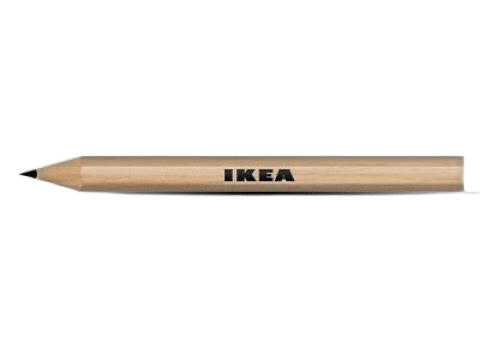
\includegraphics[scale=0.4]{ikea.png}}}{}

\vspace{-2cm}

\begin{problem}{}
В отеле бесконечное счётное количество номеров. Все номера заняты туристами.
    \begin{enumerate}
    \item[а)] Приехал еще один турист. Как разместить всех постояльцев, чтобы всем хватило места?
    \item[б)] Приехало еще счётное количество туристов. Как заново разместить всех постояльцев, чтобы всем хватило места?
    \end{enumerate}
\end{problem}
% \begin{sol}
% К сожалению, придется доставить жильцам отеля определенный дискомфорт и пересилить их в другие номера.

% \begin{center}
% 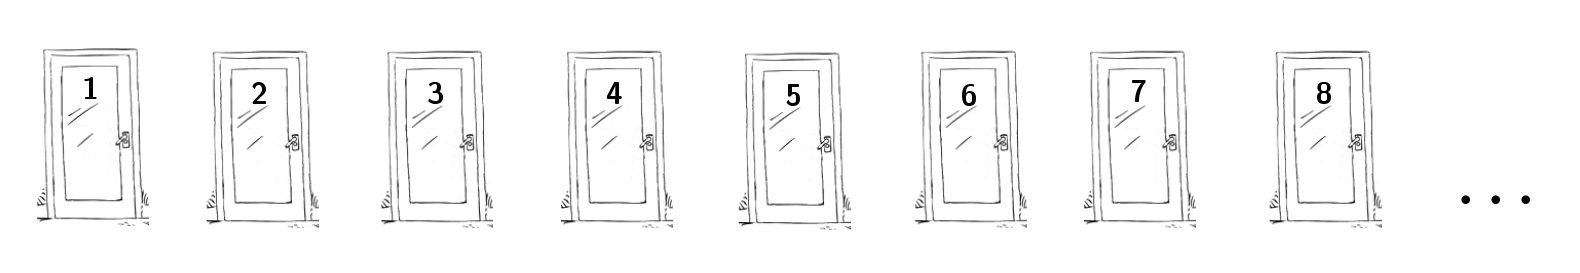
\includegraphics[scale=1.2]{door1}
% \end{center}

% \begin{enumerate}
% \item Переселим туриста из 1 номера во 2 номер, туриста из 2 номера в 3 номер, туриста из 3 номера в 4 номер и так далее. В итоге освободится место для еще одного туриста.

% \begin{center}
% 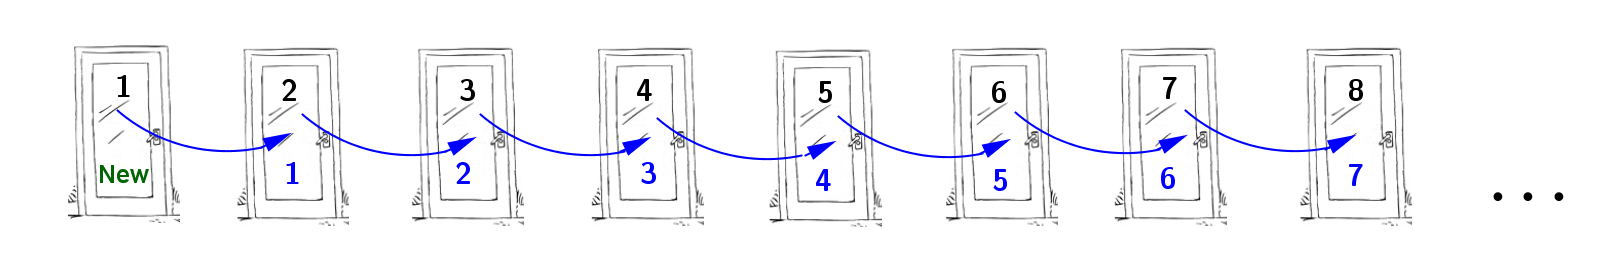
\includegraphics[scale=1.2]{door2}
% \end{center}

% \item Переселим туриста из 1 номера во 2 номер, из 2 номера в 4 номер, из 3 номера в 6 номер, из 4 номера в 8 номер, из 5 номера в 10 номер и так далее. В итоге освободится счётное количество номеров для дополнительного счётного количества туристов.

% \begin{center}
% 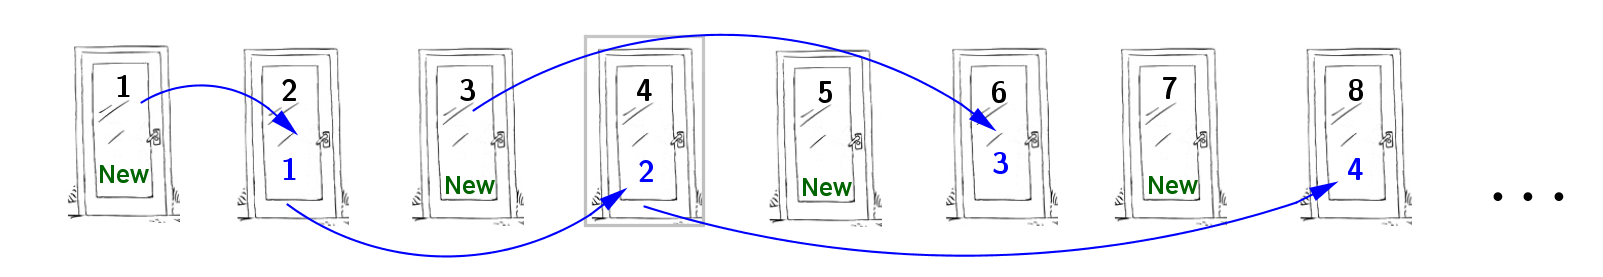
\includegraphics[scale=1.2]{door3}
% \end{center}

% \end{enumerate}

% При решении задачи мы неявно оперировали тем фактом, что если из счётного множества удалить конечное или счётное множество, то исходное множество останется счётным. Если в счётное множество добавить конечное или счётное множество, то новое множество снова будет счётным. Чтобы доказать это достаточно построить взаимно-однозначные соответствия по аналогии с тем, как мы сделали это с жильцами.
% \end{sol}


\begin{problem}{}
    Пусть $A$ --- список всех подмножеств натуральных чисел, а $S$ --- множество бесконечных последовательностей из 0 и 1. Для примера: $\{5,6,178\} \in A, \mbox{ } 0101010101010101 \ldots \in S$. Сравните мощности множеств $A$ и $S$, мощности множеств $\NN$ и $S$.
\end{problem}
% \begin{sol}
% Сопоставим каждой последовательности из нулей и единиц элемент списка $A$. Если в данный элемент списка входит  натуральное число $n$, то будем ставить в последовательности на месте $n$ единицу.

%  \begin{center}
% \definecolor{qqqqff}{rgb}{0.,0.,1.}
% \definecolor{qqttcc}{rgb}{0.,0.2,0.8}
% \definecolor{qqqqcc}{rgb}{0.,0.,0.8}
% \begin{tikzpicture}[line cap=round,line join=round,>=triangle 45,x=1cm,y=1cm]
% \clip(-0.7941728581796409,-2.9900066347568117) rectangle (10.560863242043467,3.5563131098557585);
% \draw [rotate around={90.:(2.,0.)},line width=1.6pt,color=qqqqcc] (2.,0.) ellipse (2.7489679841754673cm and 1.8859546595880108cm);
% \draw [rotate around={90.:(8,0.)},line width=1.6pt,color=qqttcc] (8,0.) ellipse (2.7489679841754686cm and 1.885954659588012cm);
% \draw [->] (2.,1.5) -- (7.5,1.5);
% \draw [->,line width=0.4pt] (7.5,1.5) -- (2.,1.5);
% \draw [->,line width=0.4pt] (2.,0.5) -- (7.5,0.5);
% \draw [->,line width=0.4pt] (7.5,0.5) -- (2.,0.5);
% \draw [->,line width=0.4pt] (2.,-0.5) -- (7.5,-0.5);
% \draw [->,line width=0.4pt] (7.5,-0.5) -- (2.,-0.5);
% \draw [->,line width=0.4pt] (2.,-1.5) -- (7.5,-1.5);
% \draw [->,line width=0.4pt] (7.5,-1.5) -- (2.,-1.5);
% \draw (1.1,1.9803472454119917) node[anchor=north west] {$\mathbf{\varnothing}$};
% \draw (0.9,0.9835825106355921) node[anchor=north west] {$\mathbf{\{1\}}$};
% \draw (0.7,-0.04012181156719667) node[anchor=north west] {$\mathbf{\{1,3\}}$};
% \draw (0.7,-1.009946958917207) node[anchor=north west] {$\mathbf{\{2,4\}}$};
% \draw (7.5,1.966877451698797) node[anchor=north west] {\small{$\mathbf{00000\ldots}$}};
% \draw (7.5,0.9701127169223975) node[anchor=north west] {\small{$\mathbf{10000\ldots}$}};
% \draw (7.5,-0.02665201785400208) node[anchor=north west] {\small{$\mathbf{10100\ldots}$}};
% \draw (7.5,-1.0503563400567908) node[anchor=north west] {\small{$\mathbf{01010\ldots}$}};
% \draw (7.7,-1.8) node[anchor=north west] {$\dots$};
% \draw (1.7,-1.8) node[anchor=north west] {$\dots$};
% \begin{scriptsize}
% \draw [fill=qqqqff] (2.,1.5) circle (2.0pt);
% \draw [fill=qqqqff] (2.,0.5) circle (2.0pt);
% \draw [fill=qqqqff] (2.,-0.5) circle (2.0pt);
% \draw [fill=qqqqff] (2.,-1.5) circle (2.0pt);
% \draw [fill=qqqqff] (7.5,1.5) circle (2.0pt);
% \draw [fill=qqqqff] (7.5,0.5) circle (2.0pt);
% \draw [fill=qqqqff] (7.5,-0.5) circle (2.0pt);
% \draw [fill=qqqqff] (7.5,-1.5) circle (2.0pt);
% \end{scriptsize}
% \end{tikzpicture}
% \end{center}

% Таким образом каждой последовательности будет соответствовать единственный элемент списка. Множества $A$ b $S$ равномощны.

% Так как мощность списка из подмножеств множества больше мощности множества и $|A|=|S|$, то $|\NN|<|S|$.
% \end{sol}


\begin{problem}{}
Аргументированно ответьте на следующие вопросы:

\begin{enumerate} 
    \item[а)] Верно ли, что если из бесконечного множества удалить счётное, то оставшаяся часть будет равномощна исходному множеству?
    \item[б)] Правда ли, что множество иррациональных чисел счётно?
    \item[в)] Сравните мощности множеств $A$ и $B$, если $A = \QQ$ --- рациональные числа, $B = \QQ^{2}$ --- пары рациональных чисел.
    \item[г)] Декартово произведение конечного количества счётных множеств
является счётным множеством. Да или нет?
    \item[д)] Правда ли, что множество всех последовательностей натуральных чисел --- множество мощности континуум? А множество вещественных числовых последовательностей --- множество мощности континуум?
\end{enumerate} 
\end{problem}
% \begin{sol}
% Да, это верно! Пусть $M$ --- бесконечное множество. Удалим из него счётные множества $B$ и $A$. Тогда с одной стороны $N = (M\setminus A)\setminus B \Rightarrow (M \setminus A) = N \cap B $. С другой стороны $N = M \setminus (B \cup A) \Rightarrow M = N \cap (A \cap B)$. Установим между множествами $M\setminus A$ и $M$ взаимно-однозначное соответствие.

% Если $x \in N$, то во множестве  $M\setminus A$ он будет соответствовать самому себе. Если же $x \in A \cap B$, то учитывая что множества $A$ и $B$ счётные, то их объединение тоже является счётным множество и можно установить взаимно-однозначное соответствие между $A \cap B$ и $B$. Таким образом каждому элементу из $M\setminus A$ соответствует единственный элемент из $M$.
% \end{sol}

% \begin{sol}
% Нет! Это враньё! Множество иррациональных чисел можно получить, выбросив из множества действительных чисел все рациональные. Полученное множество равномощно исходному.
% \end{sol}

% \begin{sol}
% $|A| <|B|$
% \end{sol}

% \begin{sol}
% Да. Все элементы этого множества можно пересчитать змейкой.
% \end{sol}

% \begin{sol}
% Да, это чистая правда в обоих случаях. Множество всех последовательностей натуральных чисел --- это ни что иное, как декартово произведение счётного числа счётных множеств. Это означает, что множество последовательностей натуральных чисел имеет мощность континуум.

% Множество всех вещественных числовых последовательностей совпадает с декартовым произведением $\RR \times \RR \times \RR \times \ldots$
% \end{sol}





% \begin{problem}{}
% \todo[inline]{Нужна норм формулировка}
% В славном городе $N$ континуальное число очень творческих жителей, которым постоянно не сидится на месте. Кто-то из них любит рисовать, кто-то петь, кто-то вышивать. Более того, в городе живут одни экстраверты, каждый из которых интересуется творчеством своих коллег. Благодаря этому у каждого горожанина существует фан-клуб, в котором состоят другие жильцы города, полюбившие его творчество. Каждый горожанин может состоять в любом количестве фан-клубов.

% Пусть $A$ --- множество горожан, а $2^A$ ---  список фан-клубов, в которых они состоят. Например, у Вовочки в фан-клубе могут состоять Паша и Артём, может состоять счётное или континуальное число жильцов, а может и вовсе никого не состоять. При этом сам Вовочка может вступить в неограниченное количество фан-клубов, или вовсе не вступить ни в один.

% \textbf{Hint:} фактически у вас просят доказать следующую теорему.Пусть $A$ произвольное множество. Докажите, что мощность множества $2^{A}$ (множество всех подмножеств множества $A$) больше, чем мощность $A$.
% \end{problem}
% \begin{sol}
% Мощность $2^{A}$ не меньше мощности $A$, т.к. есть одноточечные подмножества, которые можно сопоставить с элементами $A$. Допустим все же, что $2^{A}$ и $A$ равномощны. Значит есть взаимно однозначное соответствие $b\longleftrightarrow B$, где $b\in A$ и $B\in 2^{A}$. Построим $C\subset A$ по принципу: будем включать туда только такие $b$, которые не входят в соответствующее $B$. Этому множеству $C$ должен соответствовать некий элемент $c$. С одной стороны $c$ не может входить в $C$, с другой стороны - обязан. Противоречие.
% \end{sol}


\begin{problem}{}
Назовем две бесконечных вправо последовательности из нулей и единиц «похожими», если они отличаются на конечное число членов. Например, $101111111 \ldots$ и $000111111 \ldots$ похожа, а $101010101 \ldots$ и $010101010 \ldots$ не похожи.
    \begin{enumerate}
        \item[а)] Какова мощность множества последовательностей похожих на последовательность из одних нулей?
        \item[б)] Это отношение «похожести» разбивает все последовательности на классы похожих последовательностей. Какова мощность множества классов похожих последовательностей?
    \end{enumerate}
\end{problem}
% \begin{sol}
% Множество последовательностей «похожих» на последовательность из одних нулей будет либо счетным, либо континуальным. Среди всех этих последовательностей есть такие, которые отличаются от нулевой только первой цифрой. Есть такие, которые отличаются от нулевой первой или второй цифрой, есть такие, которые отличаются первой или второй или третьей цифрой и так далее. Все такие отличия можно занумеровать.

% \begin{center}
% \definecolor{qqqqff}{rgb}{0.,0.,1.}
% \definecolor{qqttcc}{rgb}{0.,0.2,0.8}
% \definecolor{qqqqcc}{rgb}{0.,0.,0.8}
% \begin{tikzpicture}[line cap=round,line join=round,>=triangle 45,x=1.0cm,y=1.0cm]
% \clip(-0.4849001735617755,-3.081553672504657) rectangle (10.42080979412848,3.2409971695233946);
% \draw [rotate around={90.:(2.,0.)},line width=1.6pt,color=qqqqcc] (2.,0.) ellipse (2.7489679841754673cm and 1.8859546595880108cm);
% \draw [rotate around={90.:(8.,0.)},line width=1.6pt,color=qqttcc] (8.,0.) ellipse (2.7489679841754686cm and 1.885954659588012cm);
% \draw [->] (2.,2.) -- (7.,2.);
% \draw [->,line width=0.4pt] (7.,2.) -- (2.,2.);
% \draw [->,line width=0.4pt] (2.,1.4) -- (7.,1.4);
% \draw [->,line width=0.4pt] (7.,1.4) -- (2.,1.4);
% \draw [->,line width=0.4pt] (2.,0.8) -- (7.,0.8);
% \draw [->,line width=0.4pt] (7.,0.8) -- (2.,0.8);
% \draw [->,line width=0.4pt] (2.,0.2) -- (7.,0.2);
% \draw [->,line width=0.4pt] (7.,0.2) -- (2.,0.2);
% \draw (1.3,2.381738880633563) node[anchor=north west] {$\mathbf{1}$};
% \draw (1.3,1.7881369456833312) node[anchor=north west] {$\mathbf{2}$};
% \draw (1.3,1.1945350107330993) node[anchor=north west] {$\mathbf{3}$};
% \draw (1.3,0.6009330757828673) node[anchor=north west] {$\mathbf{4}$};
% \draw (7.287143765437737,2.371301311340497) node[anchor=north west] {$\mathbf{1000 \ldots}$};
% \draw (7.287143765437737,1.7500899840669981) node[anchor=north west] {$\mathbf{0100 \ldots}$};
% \draw (7.314753157761003,1.1564880491167662) node[anchor=north west] {$\mathbf{1100 \ldots}$};
% \draw (7.300948461599369,0.549081418004901) node[anchor=north west] {$\mathbf{0010 \ldots}$};
% \draw [->,line width=0.4pt] (2.,-0.4) -- (7.,-0.4);
% \draw [->,line width=0.4pt] (7.,-0.4) -- (2.,-0.4);
% \draw (1.3,-0.07972174850936878) node[anchor=north west] {$\mathbf{5}$};
% \draw (7.480409511700602,-1.9) node[anchor=north west] {$\dots$};
% \draw (1.6134136430064763,-1.9) node[anchor=north west] {$\dots$};
% \draw [->,line width=0.4pt] (7.,-1.) -- (2.,-1.);
% \draw [->,line width=0.4pt] (7.,-1.6) -- (2.,-1.6);
% \draw [->,line width=0.4pt] (2.,-1.) -- (7.,-1.);
% \draw [->,line width=0.4pt] (2.,-1.6) -- (7.,-1.6);
% \draw (1.3,-0.6000754902792298) node[anchor=north west] {$\mathbf{6}$};
% \draw (1.3,-1.207482121391095) node[anchor=north west] {$\mathbf{7}$};
% \draw (7.300948461599369,-0.04452051694533093) node[anchor=north west] {$\mathbf{0110 \ldots}$};
% \draw (7.300948461599369,-0.6519271480571961) node[anchor=north west] {$\mathbf{1010 \ldots}$};
% \draw (7.287143765437737,-1.2455290830074282) node[anchor=north west] {$\mathbf{1110 \ldots}$};
% \begin{scriptsize}
% \draw [fill=qqqqff] (2.,2.) circle (2.0pt);
% \draw [fill=qqqqff] (2.,1.4) circle (2.0pt);
% \draw [fill=qqqqff] (2.,0.8) circle (2.0pt);
% \draw [fill=qqqqff] (2.,0.2) circle (2.0pt);
% \draw [fill=qqqqff] (7.,2.) circle (2.0pt);
% \draw [fill=qqqqff] (7.,1.4) circle (2.0pt);
% \draw [fill=qqqqff] (7.,0.8) circle (2.0pt);
% \draw [fill=qqqqff] (7.,0.2) circle (2.0pt);
% \draw [fill=qqqqff] (2.,-0.4) circle (2.0pt);
% \draw [fill=qqqqff] (7.,-0.4) circle (2.0pt);
% \draw [fill=qqqqff] (7.,-1.) circle (2.0pt);
% \draw [fill=qqqqff] (7.,-1.6) circle (2.0pt);
% \draw [fill=qqqqff] (2.,-1.) circle (2.0pt);
% \draw [fill=qqqqff] (2.,-1.6) circle (2.0pt);
% \end{scriptsize}
% \end{tikzpicture}
% \end{center}

% Таким образом последовательностей, отличающихся от нулевой счётное количество.

% Гораздо более интересным вопросом является вопрос о количестве таких счетных классов.

% \begin{center}
% \definecolor{qqttcc}{rgb}{0.,0.2,0.8}
% \definecolor{qqqqff}{rgb}{0.,0.,1.}
% \begin{tikzpicture}[line cap=round,line join=round,>=triangle 45,x=1cm,y=1cm]
% \clip(-2.5126768593015663,-2.9476257822190104) rectangle (12.312718113652455,6.872040745791953);
% \draw [rotate around={0.:(4.8,1.74)}] (4.8,1.74) ellipse (5.cm and 4.cm);
% \draw (6.5,-1.48)-- (5.52,-0.82)-- (5.84,-0.22)-- (6.14,-0.38)-- (6.68,0.44)-- (7.14,-0.3)-- (6.98,-1.14)-- (6.32,-1.02);
% \draw (5.52,-0.82)-- (6.14,-0.38);
% \draw (6.32,-1.02)-- (6.68,0.44);
% \draw (6.32,-1.02)-- (7.14,-0.3);
% \draw (6.98,-1.14)-- (6.14,-0.38);
% \draw (6.98,-1.14)-- (6.68,0.44);
% \draw (6.32,-1.02)-- (5.52,-0.82);
% \draw (6.32,-1.02)-- (5.84,-0.22);
% \draw (6.5,-1.48)-- (6.98,-1.14);
% \draw (6.5,-1.48)-- (6.32,-1.02);
% \draw (6.5,-1.48)-- (6.68,0.44);
% \draw (6.32,-1.02)-- (6.14,-0.38);
% \draw (7.14,-0.3)-- (6.14,-0.38);
% \draw (7.14,-0.3)-- (5.52,-0.82);
% \draw (7.24,2.36)-- (7.72,2.6);
% \draw (7.72,2.6)-- (8.52,2.8);
% \draw (8.52,2.8)-- (8.,3.);
% \draw (8.,3.)-- (8.02,3.5);
% \draw (8.02,3.5)-- (7.24,2.36);
% \draw (7.72,2.6)-- (8.,3.);
% \draw (7.72,2.6)-- (6.86,2.78);
% \draw (8.52,2.8)-- (6.86,2.78);
% \draw (8.,3.)-- (6.86,2.78);
% \draw (8.02,3.5)-- (6.86,2.78);
% \draw (7.24,2.36)-- (6.86,2.78);
% \draw (8.52,2.8)-- (8.64,3.48);
% \draw (8.02,3.5)-- (8.64,3.48);
% \draw (8.64,3.48)-- (8.,3.);
% \draw (8.52,2.8)-- (9.48,2.06);
% \draw (9.48,2.06)-- (9.14,2.12);
% \draw (9.14,2.12)-- (8.64,3.48);
% \draw (9.48,2.06)-- (8.02,3.5);
% \draw (9.14,2.12)-- (8.52,2.8);
% \draw (9.14,2.12)-- (8.4,2.3);
% \draw (9.14,2.12)-- (8.52,2.8);
% \draw (8.4,2.3)-- (8.52,2.8);
% \draw (8.4,2.3)-- (7.72,2.6);
% \draw (8.4,2.3)-- (8.,3.);
% \draw (8.4,2.3)-- (7.24,2.36);
% \draw (8.4,2.3)-- (8.02,3.5);
% \draw (9.14,2.12)-- (7.72,2.6);
% \draw (9.48,2.06)-- (6.86,2.78);
% \draw (2.,4.)-- (2.62,4.18);
% \draw (2.62,4.18)-- (2.46,3.12);
% \draw (2.46,3.12)-- (2.,4.);
% \draw (2.,4.)-- (1.68,3.24);
% \draw (1.68,3.24)-- (2.46,3.12);
% \draw (1.68,3.24)-- (2.62,4.18);
% \draw (2.62,4.18)-- (3.,4.);
% \draw (2.46,3.12)-- (3.,4.);
% \draw (3.,4.)-- (1.68,3.24);
% \draw (3.,4.)-- (2.,4.);
% \draw (2.46,3.12)-- (2.38,2.56);
% \draw (1.68,3.24)-- (2.38,2.56);
% \draw (3.3,3.6)-- (2.38,2.56);
% \draw (3.3,3.6)-- (3.,4.);
% \draw (3.,4.)-- (2.38,2.56);
% \draw (2.62,4.18)-- (2.38,2.56);
% \draw (2.,4.)-- (2.38,2.56);
% \draw (2.46,3.12)-- (3.3,3.6);
% \draw (2.,4.)-- (3.3,3.6);
% \draw (1.68,3.24)-- (3.3,3.6);
% \draw (-2.224991316488746,5.682940502165626) node[anchor=north west] {$\mathbf{\text{Похожи на } 01010101 \ldots }$};
% \draw [shift={(1.160814549180328,5.0314241803278685)},color=qqttcc]  plot[domain=3.262995017093252:4.779481248395654,variable=\t]({1.*2.0760950663606086*cos(\t r)+0.*2.0760950663606086*sin(\t r)},{0.*2.0760950663606086*cos(\t r)+1.*2.0760950663606086*sin(\t r)});
% \draw [->,color=qqttcc] (1.1776834965698395,2.9553976479394146) -- (1.4048299015655794,2.9657965834536766);
% \draw (7.057662198271599,6.181595443041183) node[anchor=north west] {$\mathbf{\text{Похожи на } 001001001 \ldots }$};
% \draw [->,color=qqttcc] (8.81821435797549,5.401764581633871) -- (8.525349153482352,3.736093731079142);
% \draw (7.498780030584591,-1.6434513214675532) node[anchor=north west] {$\mathbf{\text{Похожи на } 00000000 \ldots }$};
% \draw [shift={(8.011220500554714,-1.7385720252851204)},color=qqttcc]  plot[domain=0.040660055447149734:1.6090426735418257,variable=\t]({1.*1.3938763137908046*cos(\t r)+0.*1.3938763137908046*sin(\t r)},{0.*1.3938763137908046*cos(\t r)+1.*1.3938763137908046*sin(\t r)});
% \draw [->,color=qqttcc] (8.041692759200084,-0.345028836288062) -- (7.788408632794053,-0.3407829975508422);
% \begin{scriptsize}
% \draw [fill=qqqqff] (4.,5.) circle (1.0pt);
% \draw [fill=qqqqff] (3.5,4.52) circle (1.0pt);
% \draw [fill=qqqqff] (2.,4.) circle (1.0pt);
% \draw [fill=qqqqff] (2.5,4.84) circle (1.0pt);
% \draw [fill=qqqqff] (3.,4.) circle (1.0pt);
% \draw [fill=qqqqff] (2.46,3.12) circle (1.0pt);
% \draw [fill=qqqqff] (1.68,3.24) circle (1.0pt);
% \draw [fill=qqqqff] (0.94,2.46) circle (1.0pt);
% \draw [fill=qqqqff] (1.28,1.9) circle (1.0pt);
% \draw [fill=qqqqff] (1.32,1.08) circle (1.0pt);
% \draw [fill=qqqqff] (1.66,0.36) circle (1.0pt);
% \draw [fill=qqqqff] (0.64,1.18) circle (1.0pt);
% \draw [fill=qqqqff] (0.4,2.46) circle (1.0pt);
% \draw [fill=qqqqff] (0.96,3.4) circle (1.0pt);
% \draw [fill=qqqqff] (2.24,1.44) circle (1.0pt);
% \draw [fill=qqqqff] (3.56,1.9) circle (1.0pt);
% \draw [fill=qqqqff] (3.98,2.84) circle (1.0pt);
% \draw [fill=qqqqff] (3.42,5.) circle (1.0pt);
% \draw [fill=qqqqff] (2.86,2.42) circle (1.0pt);
% \draw [fill=qqqqff] (4.4,3.8) circle (1.0pt);
% \draw [fill=qqqqff] (5.4,5.06) circle (1.0pt);
% \draw [fill=qqqqff] (3.3,3.6) circle (1.0pt);
% \draw [fill=qqqqff] (4.42,4.28) circle (1.0pt);
% \draw [fill=qqqqff] (5.32,3.46) circle (1.0pt);
% \draw [fill=qqqqff] (6.,4.) circle (1.0pt);
% \draw [fill=qqqqff] (5.58,4.54) circle (1.0pt);
% \draw [fill=qqqqff] (4.8,5.26) circle (1.0pt);
% \draw [fill=qqqqff] (6.44,4.24) circle (1.0pt);
% \draw [fill=qqqqff] (6.2,5.) circle (1.0pt);
% \draw [fill=qqqqff] (7.14,3.66) circle (1.0pt);
% \draw [fill=qqqqff] (7.9,4.3) circle (1.0pt);
% \draw [fill=qqqqff] (7.04,4.68) circle (1.0pt);
% \draw [fill=qqqqff] (8.,3.) circle (1.0pt);
% \draw [fill=qqqqff] (8.02,3.5) circle (1.0pt);
% \draw [fill=qqqqff] (6.86,2.78) circle (1.0pt);
% \draw [fill=qqqqff] (5.76,3.1) circle (1.0pt);
% \draw [fill=qqqqff] (3.94,1.34) circle (1.0pt);
% \draw [fill=qqqqff] (5.,2.16) circle (1.0pt);
% \draw [fill=qqqqff] (5.68,1.4) circle (1.0pt);
% \draw [fill=qqqqff] (6.24,2.42) circle (1.0pt);
% \draw [fill=qqqqff] (5.64,2.34) circle (1.0pt);
% \draw [fill=qqqqff] (4.84,2.92) circle (1.0pt);
% \draw [fill=qqqqff] (3.96,1.84) circle (1.0pt);
% \draw [fill=qqqqff] (3.14,0.94) circle (1.0pt);
% \draw [fill=qqqqff] (2.46,0.44) circle (1.0pt);
% \draw [fill=qqqqff] (1.86,-0.36) circle (1.0pt);
% \draw [fill=qqqqff] (1.38,0.14) circle (1.0pt);
% \draw [fill=qqqqff] (0.86,0.28) circle (1.0pt);
% \draw [fill=qqqqff] (3.46,-0.72) circle (1.0pt);
% \draw [fill=qqqqff] (2.22,-1.02) circle (1.0pt);
% \draw [fill=qqqqff] (2.74,-0.02) circle (1.0pt);
% \draw [fill=qqqqff] (4.02,0.44) circle (1.0pt);
% \draw [fill=qqqqff] (2.8,-1.02) circle (1.0pt);
% \draw [fill=qqqqff] (3.6,0.14) circle (1.0pt);
% \draw [fill=qqqqff] (4.16,-0.78) circle (1.0pt);
% \draw [fill=qqqqff] (4.84,0.18) circle (1.0pt);
% \draw [fill=qqqqff] (4.5,1.) circle (1.0pt);
% \draw [fill=qqqqff] (4.5,1.74) circle (1.0pt);
% \draw [fill=qqqqff] (5.24,0.72) circle (1.0pt);
% \draw [fill=qqqqff] (4.38,-0.22) circle (1.0pt);
% \draw [fill=qqqqff] (5.52,-0.82) circle (1.0pt);
% \draw [fill=qqqqff] (5.66,0.18) circle (1.0pt);
% \draw [fill=qqqqff] (5.08,-0.18) circle (1.0pt);
% \draw [fill=qqqqff] (4.7,-1.02) circle (1.0pt);
% \draw [fill=qqqqff] (4.22,-1.78) circle (1.0pt);
% \draw [fill=qqqqff] (3.26,-1.54) circle (1.0pt);
% \draw [fill=qqqqff] (5.16,-1.9) circle (1.0pt);
% \draw [fill=qqqqff] (5.98,-1.82) circle (1.0pt);
% \draw [fill=qqqqff] (6.98,-1.14) circle (1.0pt);
% \draw [fill=qqqqff] (6.32,-1.02) circle (1.0pt);
% \draw [fill=qqqqff] (6.5,-1.48) circle (1.0pt);
% \draw [fill=qqqqff] (7.14,-0.3) circle (1.0pt);
% \draw [fill=qqqqff] (6.14,-0.38) circle (1.0pt);
% \draw [fill=qqqqff] (5.84,-0.22) circle (1.0pt);
% \draw [fill=qqqqff] (6.68,0.44) circle (1.0pt);
% \draw [fill=qqqqff] (7.62,-0.12) circle (1.0pt);
% \draw [fill=qqqqff] (7.86,-1.02) circle (1.0pt);
% \draw [fill=qqqqff] (8.58,-0.22) circle (1.0pt);
% \draw [fill=qqqqff] (8.02,0.24) circle (1.0pt);
% \draw [fill=qqqqff] (7.44,0.54) circle (1.0pt);
% \draw [fill=qqqqff] (7.,1.) circle (1.0pt);
% \draw [fill=qqqqff] (6.08,0.8) circle (1.0pt);
% \draw [fill=qqqqff] (6.76,1.52) circle (1.0pt);
% \draw [fill=qqqqff] (6.3,2.) circle (1.0pt);
% \draw [fill=qqqqff] (7.4,1.74) circle (1.0pt);
% \draw [fill=qqqqff] (7.84,1.) circle (1.0pt);
% \draw [fill=qqqqff] (8.64,0.52) circle (1.0pt);
% \draw [fill=qqqqff] (9.,0.26) circle (1.0pt);
% \draw [fill=qqqqff] (9.,1.) circle (1.0pt);
% \draw [fill=qqqqff] (8.38,1.28) circle (1.0pt);
% \draw [fill=qqqqff] (7.24,2.36) circle (1.0pt);
% \draw [fill=qqqqff] (8.4,2.3) circle (1.0pt);
% \draw [fill=qqqqff] (8.66,1.86) circle (1.0pt);
% \draw [fill=qqqqff] (7.96,1.76) circle (1.0pt);
% \draw [fill=qqqqff] (7.72,2.6) circle (1.0pt);
% \draw [fill=qqqqff] (8.52,2.8) circle (1.0pt);
% \draw [fill=qqqqff] (9.14,2.12) circle (1.0pt);
% \draw [fill=qqqqff] (9.34,1.26) circle (1.0pt);
% \draw [fill=qqqqff] (9.36,0.82) circle (1.0pt);
% \draw [fill=qqqqff] (9.48,2.06) circle (1.0pt);
% \draw [fill=qqqqff] (8.64,3.48) circle (1.0pt);
% \draw [fill=qqqqff] (8.2,4.) circle (1.0pt);
% \draw [fill=qqqqff] (6.38,3.4) circle (1.0pt);
% \draw [fill=qqqqff] (5.24,4.02) circle (1.0pt);
% \draw [fill=qqqqff] (4.44,3.16) circle (1.0pt);
% \draw [fill=qqqqff] (3.8,3.52) circle (1.0pt);
% \draw [fill=qqqqff] (3.36,2.52) circle (1.0pt);
% \draw [fill=qqqqff] (2.38,2.56) circle (1.0pt);
% \draw [fill=qqqqff] (1.26,2.34) circle (1.0pt);
% \draw [fill=qqqqff] (2.34,2.12) circle (1.0pt);
% \draw [fill=qqqqff] (1.44,3.8) circle (1.0pt);
% \draw [fill=qqqqff] (1.68,4.52) circle (1.0pt);
% \draw [fill=qqqqff] (0.28,1.8) circle (1.0pt);
% \draw [fill=qqqqff] (0.86,-0.24) circle (1.0pt);
% \draw [fill=qqqqff] (1.64,-0.98) circle (1.0pt);
% \draw [fill=qqqqff] (0.34,0.74) circle (1.0pt);
% \draw [fill=qqqqff] (4.48,4.66) circle (1.0pt);
% \draw [fill=qqqqff] (2.62,4.18) circle (1.0pt);
% \end{scriptsize}
% \end{tikzpicture}
% \end{center}

% Допустим, что классов счётное количество. Тогда объединение всех классов должно дать все возможные последовательности из нулей и единиц. Счётное объединение счётного количества множеств --- счётное множество, а множество последовательностей из нулей и единиц, в свою очередь --- континуальное множество, значит множество классов не может быть счётным и является континуальным.
% \end{sol}


\begin{problem}{}
Злобный Дракон поймал бесконечное счётное количество гномов. Расставил их в шеренгу так, что первый видят всех остальных, второй --- всех, начиная с третьего гнома, третий --- всех, начиная с четвертого и т.д. Далее Дракон надевает каждому гному либо чёрный, либо белый колпак.

\begin{center}
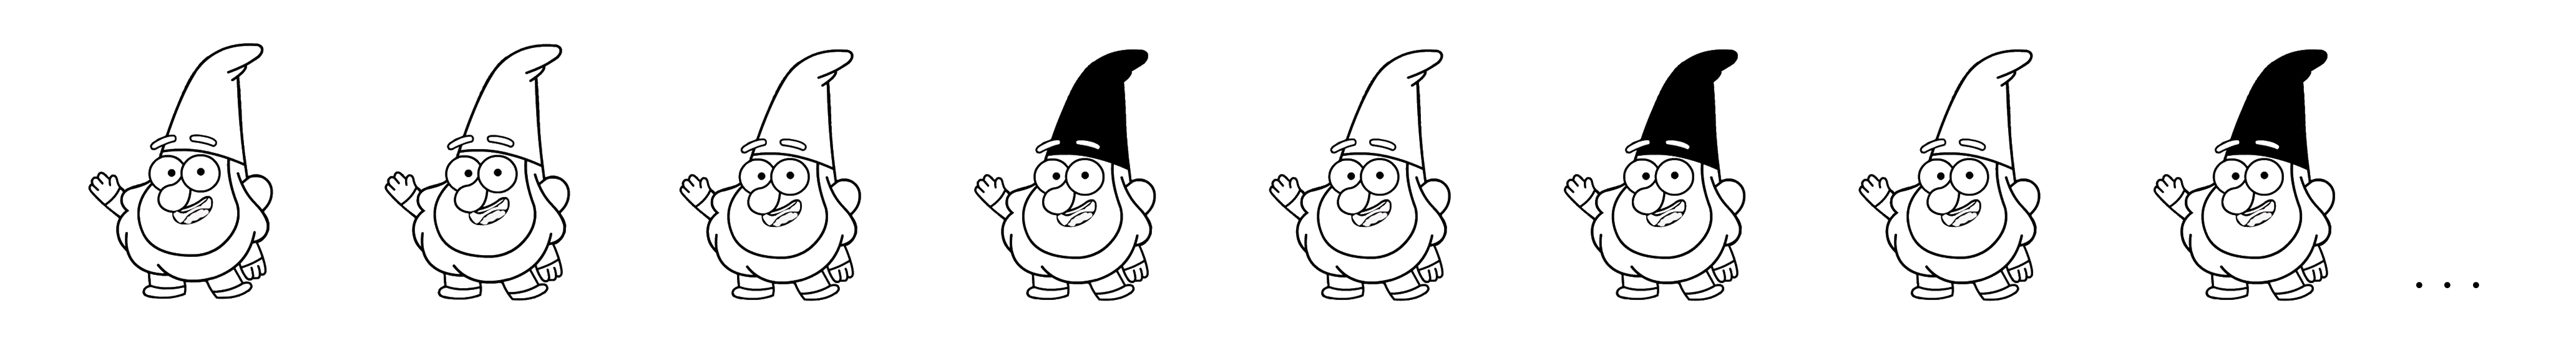
\includegraphics[scale=0.5]{dwarfs}
\end{center}

 Гномы одновременно пытаются угадать цвет своего колпака. Гномы, не угадавшие цвет своего колпака, съедаются Драконом. Есть ли у гномов\footnote{Подробнее о гномах, изображенных на картинке можно узнать, например, по ссылке \url{http://gravityfalls.ru/}} стратегия, позволяющая им иметь конечные боевые потери при встрече со Злобным Драконом?

\textbf{Hints:} Воспользуйтесь результатом из предыдущей задачи!
\end{problem}
% \begin{sol}
% Пусть чёрные колпаки --- единица, а белые колпаки --- ноль. В этом случае дракон, надевая на гномов колпаки создает бесконечную последовательность из нулей и единиц. Созданная последовательность будет относится к какому-то определенному классу «похожих» --- отличающихся в счетном числе точек последовательностей.

% Гномам, чтобы потерять конечное число своих собратьев необходимо заранее из каждого класса выбрать образцовую последовательность.

% Глядя на колпаки впереди стоящих гномов можно идентифицировать класс, которому принадлежит фактическая последовательность колпаков.

% Первый гном, поняв к какому классу относится последовательность, назовет первый элемент образцовой последовательности. Второй гном назовет второй и так далее. Так как все последовательности одного класса различаются в конечном числе точек, то погибнет конечное число гномов.
% \end{sol}


\begin{problem}{}
Злобный Дракон поймал всего лишь $n$ гномов. Расставил их в шеренгу так, что первый видят всех остальных, второй --- всех, начиная с третьего гнома, третий --- всех, начиная с четвертого и т.д. Далее Дракон надевает каждому гному либо чёрный, либо белый колпак. Гномы одновременно пытаются угадать цвет своего колпака. Гномы, не угадавшие цвет своего колпака, съедаются Драконом. Есть ли у гномов какая-то оптимальная стратегия, которая позволит противостоять дракону? Сколько гномов погибнет в лучшем и в худшем исходах?
\end{problem}
% \begin{sol}
% Пусть чёрные колпаки --- единица, а белые колпаки --- ноль. В этом случае дракон, надевая на гномов колпаки создает конечную последовательность из нулей и единиц. Сумма всех чисел в последовательности будет либо чётной либо нечётной.

% Первый гном видит всех остальных. Если количество белых колпаков перед ним чётное, он называет белый цвет. Если количество нечетноё, чёрный. Если первый гном назвал белый цвет, а второй гном видит перед собой чётное количество белых колпаков, то он делает вывод, что на нём одет чёрный колпак. Остальные гномы внимательно анализируют что именно скажет их товарищ, стоящий за их спиной и выживают.

% При этом, если первый гном угадает цвет своего колпака, то никто не погибнет.
% \end{sol}


\begin{problem}{}
Постройте взаимно-однозначное соответствие между множествами $(0;1) \times (0;1)$ и $\RR^{2}$. С помощью построенного соответствия докажите, что множества $[0;1] \times [0;1]$ и $\RR^{2}$ равномощны.
\end{problem}


% \begin{sol}
% Для того, чтобы каждому элементу из множества $(0;1) \times (0;1)$ поставить единственным образом в соответствие элемент из $\RR^{2}$ нужно найти такое отображение, что:
% \[ \lim_{x \to 0} f(x) = - \infty \text{ и } \lim_{x \to 1} f(x) = + \infty.\] Аналогичное отображение нужно подобрать для переменной $y$. Первое, что приходит в голову --- начать экспериментировать с экспонентами и тангенсами, но это плохая идея.

% Попробуем не заморачиваться. Чтобы $\lim_{x \to 0} f(x) = - \infty$ достаточно взять функцию $-\dfrac{1}{x^2}$. Чтобы получить  $\lim_{x \to 1} f(x) = + \infty$ достаточно взять функцию $\dfrac{1}{(x-1)^2}$. Тогда для функции $-\dfrac{1}{x^2} + \dfrac{1}{(x-1)^2}$ получаем:

% \[\lim_{x \to 0} \left(-\frac{1}{x^2} + \dfrac{1}{(x-1)^2}\right) = -\infty -1 = -\infty,\]

% \[\lim_{x \to 1} \left(-\frac{1}{x^2} + \dfrac{1}{(x-1)^2}\right) = -1 + \infty = +\infty,\].

% Таким образом по правилу $(x,y) \leftrightarrow \left(-\dfrac{1}{x^2} + \dfrac{1}{(x-1)^2},-\dfrac{1}{y^2} + \dfrac{1}{(y-1)^2}\right)$ мы каждому элементу из $(0;1) \times (0;1)$ поставим в соответствие элемент из $\RR^{2}$.

% Для того, чтобы доказать, что множества $[0;1] \times [0;1]$ и $\RR^{2}$ равномощны, нам нужно построить взаимно-однозначное соответствие между этими двумя множествами.

% \begin{center}
% \definecolor{qqqqff}{rgb}{0.,0.,1.}
% \definecolor{qqwuqq}{rgb}{0.,0.39215686274509803,0.}
% \definecolor{ffqqqq}{rgb}{1.,0.,0.}
% \begin{tikzpicture}[line cap=round,line join=round,>=triangle 45,x=0.8cm,y=0.8cm]
% \clip(-4.111289704910403,-1.5128932941321722) rectangle (10.605912648926926,6.79873266366131);
% \fill[line width=1.6pt,color=qqwuqq,fill=qqwuqq,fill opacity=0.1] (0.,4.) -- (0.,1.) -- (-3.,1.) -- (-3.,4.) -- cycle;
% \fill[color=qqqqff,fill=qqqqff,fill opacity=0.1] (5.94,5.76) -- (4.66,5.58) -- (3.4,5.16) -- (3.06,4.02) -- (3.06,2.74) -- (2.94,1.7) -- (3.,0.82) -- (3.46,-0.18) -- (4.18,-0.74) -- (5.4,-0.84) -- (6.96,-0.9) -- (7.98,-0.42) -- (8.7,0.5) -- (9.18,1.76) -- (9.4,3.16) -- (9.18,4.4) -- (8.58,5.26) -- (7.58,5.7) -- (6.5,5.72) -- cycle;
% \draw [line width=1.6pt,color=qqwuqq] (0.,4.)-- (0.,1.);
% \draw [line width=1.6pt,color=qqwuqq] (0.,1.)-- (-3.,1.);
% \draw [line width=1.6pt,color=qqwuqq] (-3.,1.)-- (-3.,4.);
% \draw [line width=1.6pt,color=qqwuqq] (-3.,4.)-- (0.,4.);
% \draw [line width=1.6pt,dash pattern=on 8pt off 8pt,color=qqqqff] (6.059421412128413,5.75334642883689)-- (6.06,-0.84);
% \draw (-3.1,3.0178802542890866) node[anchor=north west] {$\mathbf{[0;1] \times [0;1]}$};
% \draw (3.9816092539937755,2.142972258731878) node[anchor=north west] {$\mathbf{\RR^2}$};
% \draw [->,line width=0.4pt,color=qqwuqq] (-3.,4.) -- (0.015114492880381025,3.969771014239238);
% \draw [->,line width=0.4pt,color=qqwuqq] (0.015114492880381183,0.9697710142392378) -- (0.015114492880381185,3.969771014239238);
% \begin{scriptsize}
% \draw [fill=ffqqqq] (0.,4.) circle (2.5pt);
% \end{scriptsize}
% \end{tikzpicture}
% \end{center}

% В предыдущем пункте задачи мы нашли отображение, которое переводит все точки квадрата в точки плоскости, но при этом мы не нашли ни одной точки, которой в соответствие можно было бы поставить границу квадрата. Возьмем на плоскости произвольную прямую. Прямая равномощна полупрямой с выколотым началом. То есть между ними можно установить взаимно-однозначное соответствие.

% \begin{center}
% \definecolor{wwqqzz}{rgb}{0.4,0.,0.6}
% \definecolor{qqqqff}{rgb}{0.,0.,1.}
% \definecolor{qqwuqq}{rgb}{0.,0.39215686274509803,0.}
% \definecolor{ffqqqq}{rgb}{1.,0.,0.}
% \begin{tikzpicture}[line cap=round,line join=round,>=triangle 45,x=0.8cm,y=0.8cm]
% \clip(-3.525776137780285,-1.4871732097146722) rectangle (11.158053875118634,6.026209026184774);
% \fill[line width=1.6pt,color=qqwuqq,fill=qqwuqq,fill opacity=0.1] (0.,4.) -- (0.,1.) -- (-3.,1.) -- (-3.,4.) -- cycle;
% \fill[color=qqqqff,fill=qqqqff,fill opacity=0.1] (5.94,5.76) -- (4.66,5.58) -- (3.4,5.16) -- (3.06,4.02) -- (3.06,2.74) -- (2.94,1.7) -- (3.,0.82) -- (3.46,-0.18) -- (4.18,-0.74) -- (5.4,-0.84) -- (6.96,-0.9) -- (7.98,-0.42) -- (8.7,0.5) -- (9.18,1.76) -- (9.4,3.16) -- (9.18,4.4) -- (8.58,5.26) -- (7.58,5.7) -- (6.5,5.72) -- cycle;
% \draw [line width=1.6pt,color=qqwuqq] (0.,4.)-- (0.,1.);
% \draw [line width=1.6pt,color=qqwuqq] (0.,1.)-- (-3.,1.);
% \draw [line width=1.6pt,color=qqwuqq] (-3.,1.)-- (-3.,4.);
% \draw [line width=1.6pt,color=qqwuqq] (-3.,4.)-- (0.,4.);
% \draw (-3.1,3.0178802542890866) node[anchor=north west] {$\mathbf{[0;1] \times [0;1]}$};
% \draw (3.9816092539937755,2.142972258731878) node[anchor=north west] {$\mathbf{\RR^2}$};
% \draw [line width=1.6pt,dotted,color=wwqqzz] (5.9813989581245375,2.04923211635075)-- (5.9813989581245375,5.673850955087756);
% \draw [->,line width=1.6pt,dash pattern=on 8pt off 8pt,color=qqqqff] (6.012485672022963,-0.8729189901012959) -- (5.981398958124537,2.049232116350843);
% \draw [->,line width=0.4pt,color=qqwuqq] (-3.,4.) -- (0.015114492880381025,3.969771014239238);
% \draw [->,line width=0.4pt,color=qqwuqq] (0.015114492880381183,0.9697710142392378) -- (0.015114492880381185,3.969771014239238);
% \begin{scriptsize}
% \draw [fill=ffqqqq] (0.,4.) circle (2.5pt);
% \end{scriptsize}
% \end{tikzpicture}
% \end{center}

% Любой интервал равномощен полупрямой. Сопоставим между собой границу квадрата и незанятую полупрямую с включённым началом.

% \begin{center}
% \definecolor{qqqqff}{rgb}{0.,0.,1.}
% \definecolor{qqwuqq}{rgb}{0.,0.39215686274509803,0.}
% \definecolor{ffqqqq}{rgb}{1.,0.,0.}
% \begin{tikzpicture}[line cap=round,line join=round,>=triangle 45,x=0.8cm,y=0.8cm]
% \clip(-3.579776155240749,-1.1806060881890135) rectangle (9.949582062279424,5.964416424276412);
% \fill[line width=1.6pt,color=qqwuqq,fill=qqwuqq,fill opacity=0.1] (0.015114492880381185,3.969771014239238) -- (0.015114492880381185,0.969771014239238) -- (-3.,1.) -- (-3.,4.) -- cycle;
% \fill[color=qqqqff,fill=qqqqff,fill opacity=0.1] (5.94,5.76) -- (4.66,5.58) -- (3.4,5.16) -- (3.06,4.02) -- (3.06,2.74) -- (2.94,1.7) -- (3.,0.82) -- (3.46,-0.18) -- (4.18,-0.74) -- (5.4,-0.84) -- (6.96,-0.9) -- (7.98,-0.42) -- (8.7,0.5) -- (9.18,1.76) -- (9.4,3.16) -- (9.18,4.4) -- (8.58,5.26) -- (7.58,5.7) -- (6.5,5.72) -- cycle;
% \draw [line width=1.6pt,color=qqwuqq] (0.015114492880381185,3.969771014239238)-- (0.015114492880381185,0.969771014239238);
% \draw [line width=1.6pt,color=qqwuqq] (0.015114492880381185,0.969771014239238)-- (-3.,1.);
% \draw [line width=1.6pt,color=qqwuqq] (-3.,1.)-- (-3.,4.);
% \draw [line width=1.6pt,color=qqwuqq] (-3.,4.)-- (0.015114492880381185,3.969771014239238);
% \draw (-3.1,3.0178802542890866) node[anchor=north west] {$\mathbf{[0;1] \times [0;1]}$};
% \draw (3.9816092539937755,2.142972258731878) node[anchor=north west] {$\mathbf{\RR^2}$};
% \draw [->,line width=1.6pt,dash pattern=on 7pt off 7pt,color=qqqqff] (6.012485672022963,-0.8729189901012959) -- (5.981398958124537,2.049232116350843);
% \draw [->,line width=0.4pt,color=qqwuqq] (-3.,4.) -- (0.015114492880381025,3.969771014239238);
% \draw [->,line width=0.4pt,color=qqwuqq] (0.015114492880381183,0.9697710142392378) -- (0.015114492880381185,3.969771014239238);
% \draw [->,line width=1.6pt,color=qqwuqq] (5.98314370935182,5.7470773364447645) -- (6.,2.);
% \begin{scriptsize}
% \draw [fill=ffqqqq] (0.015114492880381185,3.969771014239238) circle (2.5pt);
% \draw [fill=ffqqqq] (6.,2.) circle (2.5pt);
% \end{scriptsize}
% \end{tikzpicture}
% \end{center}

% Проделав всё это мы сопоставили плоскости квадрат с его границей. Заметим, что, используя это отображение, можно доказать равномощность $[0;1]$ и $\RR$.
% \end{sol}

\end{document} % 